\section{Resultados parciales}
\label{sec:resultados}

Las pruebas disponibles cubren progresivamente la cadena, desde el acondicionamiento hasta el registro de campo. Los barridos eléctricos verificaron continuidad, ganancia y fase de las rutas internas hasta el ADC. Al combinar la transferencia medida con el modelo nominal del SM-24, la figura~\ref{fig:caracterizacion-electrica} muestra la respuesta esperada del conjunto geófono--electrónica. La comparación distingue el resultado medido de la electrónica de la predicción que incorpora al transductor.

La calibración automática corrigió la continua etapa por etapa antes de adquirir. Las señales de la figura~\ref{fig:calibracion-etapas} convergen hacia sus referencias y los códigos obtenidos se conservan por configuración de ganancia. Una vez calibrado el frente, el PSoC digitaliza y traslada las muestras por las rutas DMA de la figura~\ref{fig:hardware-digital}; la comunicación y la interfaz operan después sobre una captura que ya quedó almacenada localmente.

La coordinación inalámbrica se ensayó de manera exploratoria con tres nodos esclavos. Durante 128 órdenes START se observaron en osciloscopio los flancos GPIO generados por los ESP32 al ejecutar la orden. La separación entre esos marcadores se encontró aproximadamente entre 200 y \SI{400}{\micro s}. El resultado demuestra la operación multiesclavo y proporciona una primera magnitud del arranque distribuido; no mide todavía el inicio efectivo de los ADC ni la deriva de sus relojes.

\begin{figure*}[!tb]
\centering
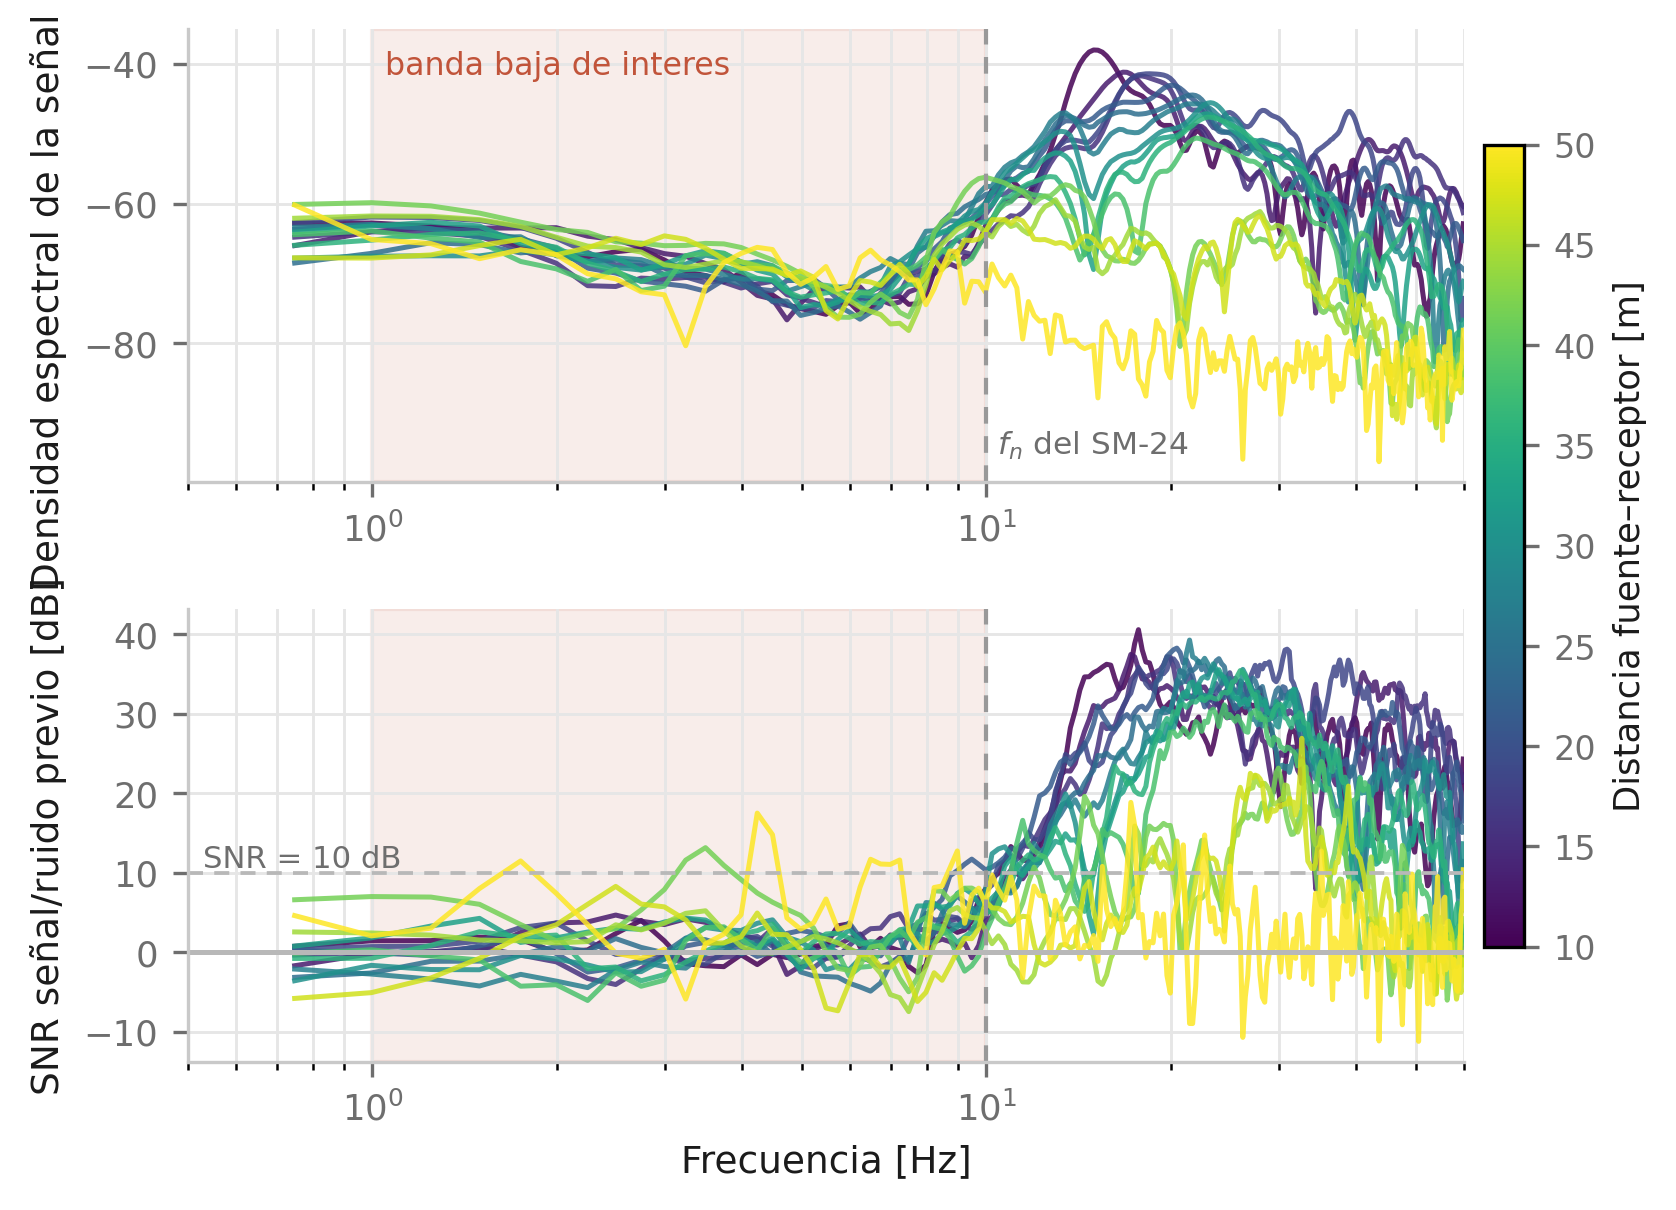
\includegraphics[width=0.64\textwidth,keepaspectratio]{f_contenido_baja_frecuencia.png}
\caption{Densidad espectral y relación señal--ruido de las capturas, agrupadas por distancia. La zona sombreada identifica la banda baja de interés y la línea vertical la frecuencia natural nominal del SM-24.}
\label{fig:contenido-baja}
\end{figure*}

\subsection{Contenido espectral de las capturas}

Para estimar la banda realmente observable se comparó, por impacto, una ventana posterior al marcador con una ventana de ruido previa. La figura~\ref{fig:contenido-baja} reúne 265 impactos en 15 distancias con al menos tres registros utilizables. La mediana de la relación señal--ruido fue 0,5 dB entre 1 y 5 Hz y 2,1 dB entre 5 y 10 Hz; aumentó a 16,7 dB entre 10 y 20 Hz y a 24,4 dB entre 20 y 50 Hz. Ninguna de las 15 distancias superó 10 dB de mediana por debajo de 10 Hz.

El resultado es extremo a extremo y, por ello, combina fuente, acoplamiento, terreno, geófono y electrónica: no permite atribuir la limitación a un único bloque. Sí establece una decisión experimental inmediata. Aumentar la energía y la repetibilidad de la excitación en baja frecuencia es necesario para evaluar cuánto puede aprovecharse la compensación del receptor y para extender la banda útil del registro.

\subsection{Registro espacial sintetizado}

La campaña desplazó un receptor entre 21 posiciones de 10 a \SI{50}{m}, con un paso de \SI{2}{m}. En cada posición se repitió el impacto, se alinearon las capturas con la referencia del martillo y se obtuvo una traza representativa. El resultado se ordenó por distancia para formar el waterfall de la figura~\ref{fig:waterfall}.

\begin{figure*}[!tb]
\centering
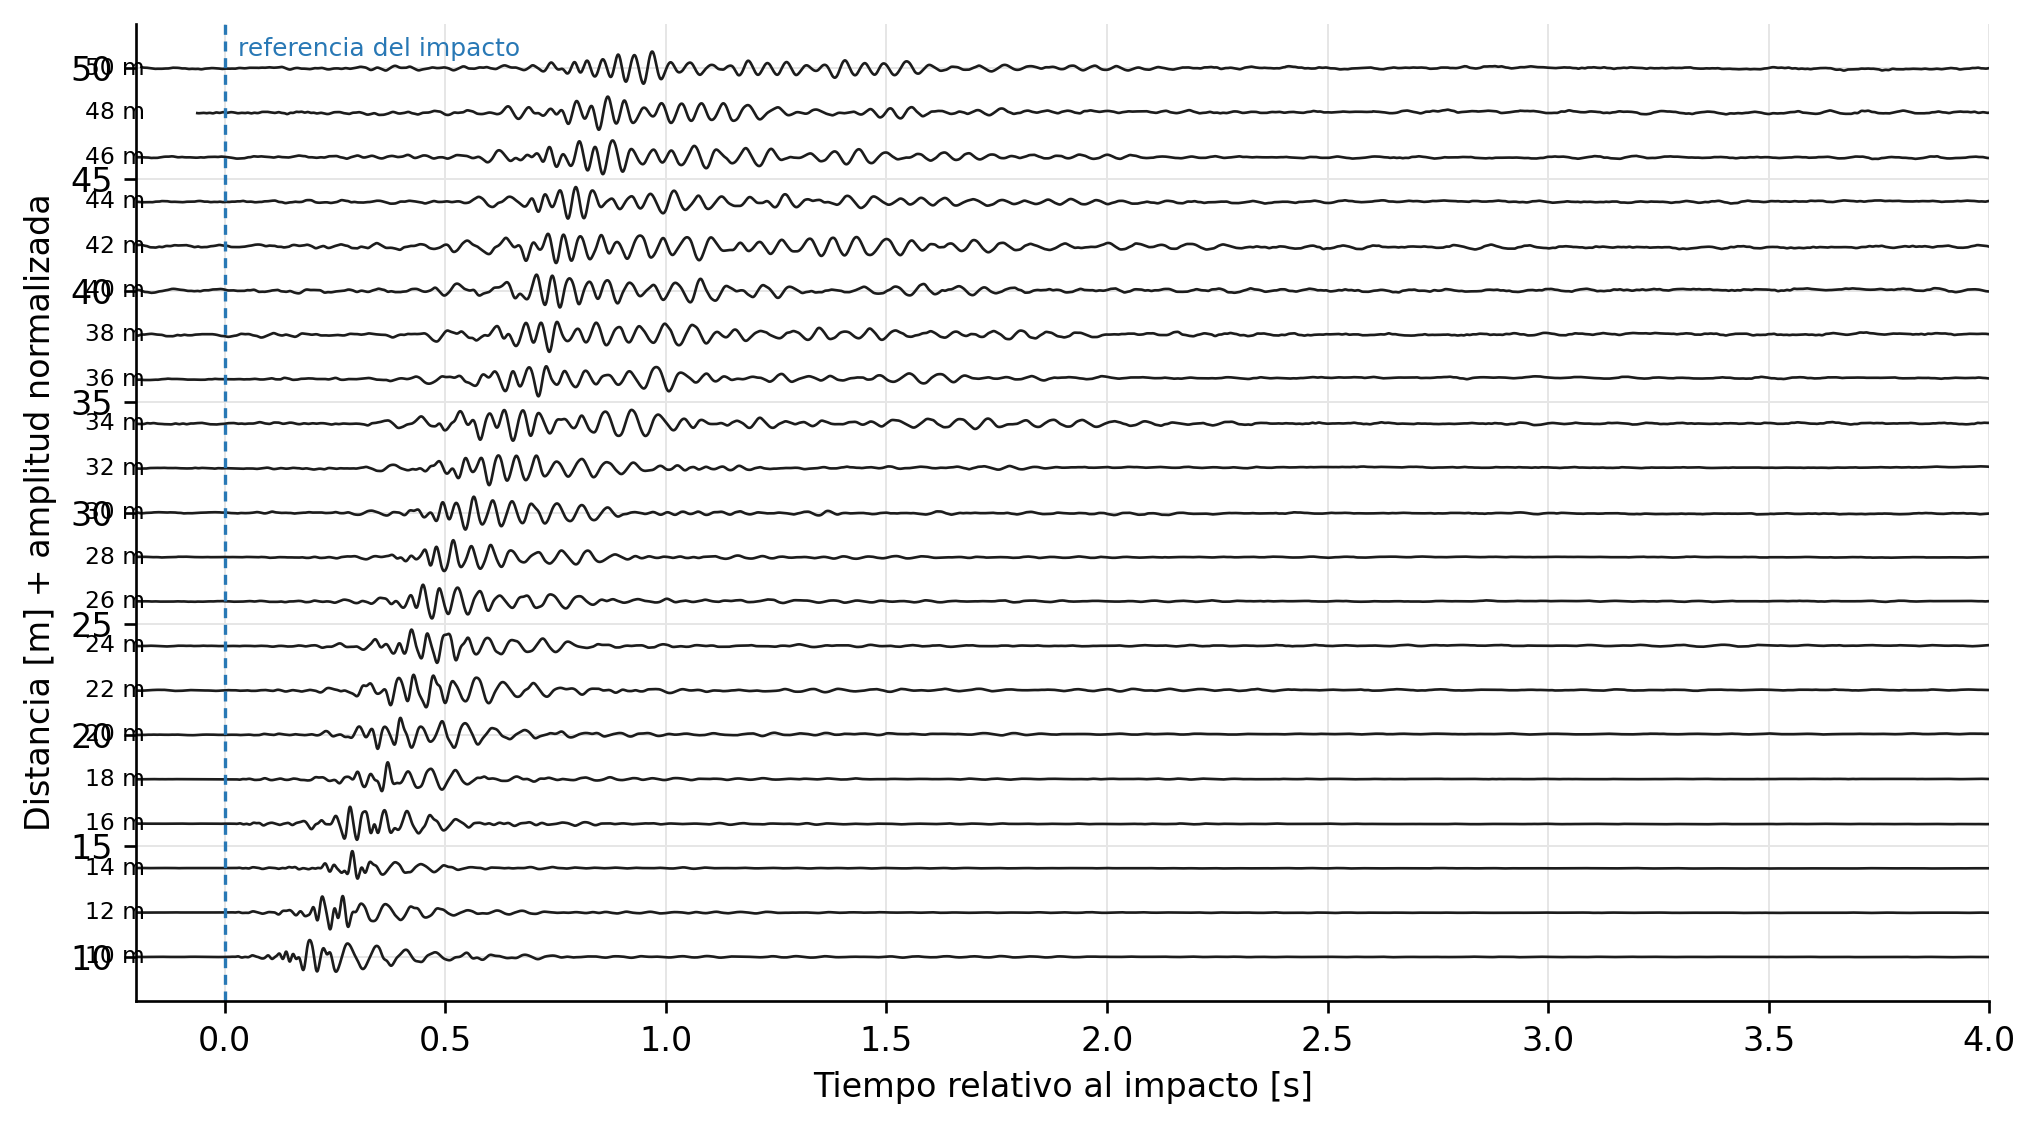
\includegraphics[width=0.67\textwidth,keepaspectratio]{f_waterfall_4s.png}
\caption{Waterfall sintetizado con 21 posiciones secuenciales y un único receptor desplazado. Se muestran los primeros 4 s posteriores al impacto; cada traza está normalizada para visualizar su evolución temporal.}
\label{fig:waterfall}
\end{figure*}

La progresión temporal observada entre posiciones confirma que la plataforma y el flujo de procesamiento permiten construir un registro espacio--tiempo. No corresponde a 21 receptores simultáneos: cada fila procede de una excitación distinta y la normalización impide comparar amplitudes absolutas. La evidencia alcanzada sostiene la afirmación central de esta etapa: se desarrolló una plataforma orientada a MASW, verificada parcialmente mediante ensayos de sus subsistemas y evidencia preliminar de campo.

\begin{table*}[!tb]
\centering
\footnotesize
\caption{Alcance de las evidencias presentadas.}
\begin{tabularx}{0.94\textwidth}{@{}lYY@{}}
\toprule
Evidencia & Qué permite afirmar & Qué no establece todavía \\
\midrule
Barridos eléctricos & Transferencia de las rutas internas y continuidad hasta el ADC & Calibración mecánica del geófono completo \\
Calibración de continua & Ajuste automático por etapa antes de adquirir & Igualdad de respuesta entre varios receptores \\
Tres esclavos, 128 START & Operación distribuida y marcadores GPIO separados aproximadamente 200--400 $\mu$s & Inicio y deriva de los ADC \\
Espectros de campo & SNR insuficiente bajo 10 Hz en el conjunto observado & Causa única de la pérdida de energía \\
Waterfall secuencial & Registro espacio--tiempo de 21 posiciones sintetizadas & Adquisición simultánea o caracterización geotécnica final \\
\bottomrule
\end{tabularx}
\label{tab:alcance-resultados}
\end{table*}

\section{Trabajo futuro}

Se fijan cuatro hitos verificables. Primero se construirá o incorporará una fuente más energética y repetible, cuya mejora se evaluará repitiendo el análisis espectral y comparando energía y SNR por banda. Segundo, una misma señal analógica se aplicará a varios nodos GEO para medir sobre los datos ADC el desfase inicial, la deriva temporal y las diferencias de ganancia y fase. Tercero, esos resultados se utilizarán para calibrar la respuesta relativa de los receptores y validar la adquisición simultánea.

Finalmente se ampliará el arreglo si se obtienen recursos para más sensores; en caso contrario se continuará con adquisición secuencial, mejorando la fuente y la trazabilidad de cada posición. Una vez consolidado el registro se estudiarán rigurosamente la formación de imágenes de dispersión, la selección modal y los algoritmos de inversión. Esas etapas pertenecen a la segunda presentación y no se utilizan aquí para atribuir propiedades geotécnicas al emplazamiento.

La evaluación de la nueva fuente conservará una geometría fija y un número definido de repeticiones. Se compararán el espectro del impacto, la energía recibida y la SNR por bandas, además de la variación entre golpes. El objetivo no será sólo elevar la amplitud total, sino demostrar una mejora reproducible en la banda baja sin saturar el frente analógico. También se registrarán las condiciones de acoplamiento para separar, en lo posible, cambios de la fuente y del montaje.

La validación multinodo seguirá un protocolo común de tasa, ganancia y duración. A partir de la señal compartida se estimará el retardo inicial entre secuencias ADC, su evolución durante la ventana y las diferencias de magnitud y fase. Se repetirán las mediciones después de rearmar los nodos para informar dispersión e incertidumbre, no únicamente un caso favorable. Sólo después de cumplir esos controles se comparará un arreglo simultáneo con el registro secuencial; ambos recorridos permanecerán disponibles porque responden a disponibilidades instrumentales distintas.

El cierre de esta etapa exigirá resultados reproducibles y trazables. Para la fuente se informarán la distribución por bandas y la variación entre repeticiones; para los receptores, los errores relativos antes y después de calibrar; y para la coordinación, el retardo y la deriva calculados directamente sobre las muestras. Estos criterios evitarán confundir el funcionamiento de la comunicación con una sincronización metrológica y permitirán decidir, con evidencia, si el sistema está listo para procesar dispersión.
